\documentclass[]{article}
\usepackage{amsmath}
\usepackage{amsfonts}
\usepackage{amssymb}
\usepackage{listings}
\usepackage{xcolor}
\usepackage{graphicx}
\usepackage{hyperref}
\usepackage{cancel}
\usepackage{algpseudocode}
\usepackage{capt-of}

\definecolor{codegreen}{rgb}{0,0.6,0}
\definecolor{codegray}{rgb}{0.5,0.5,0.5}
\definecolor{codepurple}{rgb}{0.58,0,0.82}
\definecolor{backcolour}{rgb}{0.95,0.95,0.92}

\lstdefinestyle{mystyle}{
	backgroundcolor=\color{backcolour},   
	commentstyle=\color{codegreen},
	keywordstyle=\color{magenta},
	numberstyle=\tiny\color{codegray},
	stringstyle=\color{codepurple},
	basicstyle=\ttfamily\footnotesize,
	breakatwhitespace=false,         
	breaklines=true,                 
	captionpos=b,                    
	keepspaces=true,                 
	numbers=left,                    
	numbersep=5pt,                  
	showspaces=false,                
	showstringspaces=false,
	showtabs=false,                  
	tabsize=2
}

\lstset{style=mystyle}
%opening
\title{CPSC532W Homework 5}
\author{Justin Reiher\\ Student ID: 37291151\\ CWL: reiher}
\date{}

\begin{document}

\maketitle

Link to public repository for homework 5:
\begin{center}
	\url{https://github.com/justinreiher/probProg_Fall2021/tree/main/CS532-HW5}
\end{center}

The HOPPL is implemented following Peter Norvig's tutorial \url{https://norvig.com/lispy.html} very closely. Particularly the \texttt{Procedure} and \texttt{Environment} classes:
\lstinputlisting[language = Python, linerange ={26-40}]{evaluator.py}
The evaluator itself likewise follows the format and style in the tutorial augmented with \texttt{sample} and \texttt{observe} where \texttt{observe} in this case does nothing interesting other than return the observed value:
\lstinputlisting[language = Python, linerange ={44-81}]{evaluator.py}

\section{Program 1: Deterministic and Probabilistic Tests}
Output demonstrating all tests pass:
\begin{verbatim}
FOPPL Tests passed
FOPPL Tests passed
FOPPL Tests passed
FOPPL Tests passed
FOPPL Tests passed
FOPPL Tests passed
FOPPL Tests passed
FOPPL Tests passed
FOPPL Tests passed
FOPPL Tests passed
FOPPL Tests passed
FOPPL Tests passed
FOPPL Tests passed
Test passed
Test passed
Test passed
Test passed
Test passed
Test passed
Test passed
Test passed
Test passed
Test passed
Test passed
/home/justin/Research/Research/ProbProg/CS532-HW5/primitives.py:244: UserWarning: To copy construct from a tensor, it is recommended to use sourceTensor.clone().detach() or sourceTensor.clone().detach().requires_grad_(True), rather than torch.tensor(sourceTensor).
return torch.cat((torch.tensor([val]),torch.tensor(l)),0)
Test passed
All deterministic tests passed
('normal', 5, 1.4142136)
p value 0.4392251209556768
('beta', 2.0, 5.0)
p value 0.20362142284502927
('exponential', 0.0, 5.0)
p value 0.4026319736237799
('normal', 5.3, 3.2)
p value 0.6117760761512494
('normalmix', 0.1, -1, 0.3, 0.9, 1, 0.3)
p value 0.42402962493527685
('normal', 0, 1.44)
p value 0.018257659736088516
All probabilistic tests passed	
\end{verbatim}
The warning in the HOPPL test 12:
\begin{verbatim}
/home/justin/Research/Research/ProbProg/CS532-HW5/primitives.py:244: UserWarning: To copy construct from a tensor, it is recommended to use sourceTensor.clone().detach() or sourceTensor.clone().detach().requires_grad_(True), rather than torch.tensor(sourceTensor).
return torch.cat((torch.tensor([val]),torch.tensor(l)),0)
\end{verbatim}
is telling me that I should not call \texttt{torch.tensor(l)} on a tensor object that already exists. However the behaviour is correct, which is to say that if the list is not a \texttt{torch.tensor(l)} it will create one, if it already exists then it returns the same list.
\section{Running Programs}
All programs are run with 10k samples and the results are shown below
\subsection{Program 1}
Output from running program 1:
\begin{verbatim}
Sample of prior of program 1:
Elapsed time for program  1 .daphne is:  0:05:11.798638  seconds
Mean of samples:  tensor(99.1019)
Variance of samples:  tensor(9923.6123)
\end{verbatim}
\begin{center}
	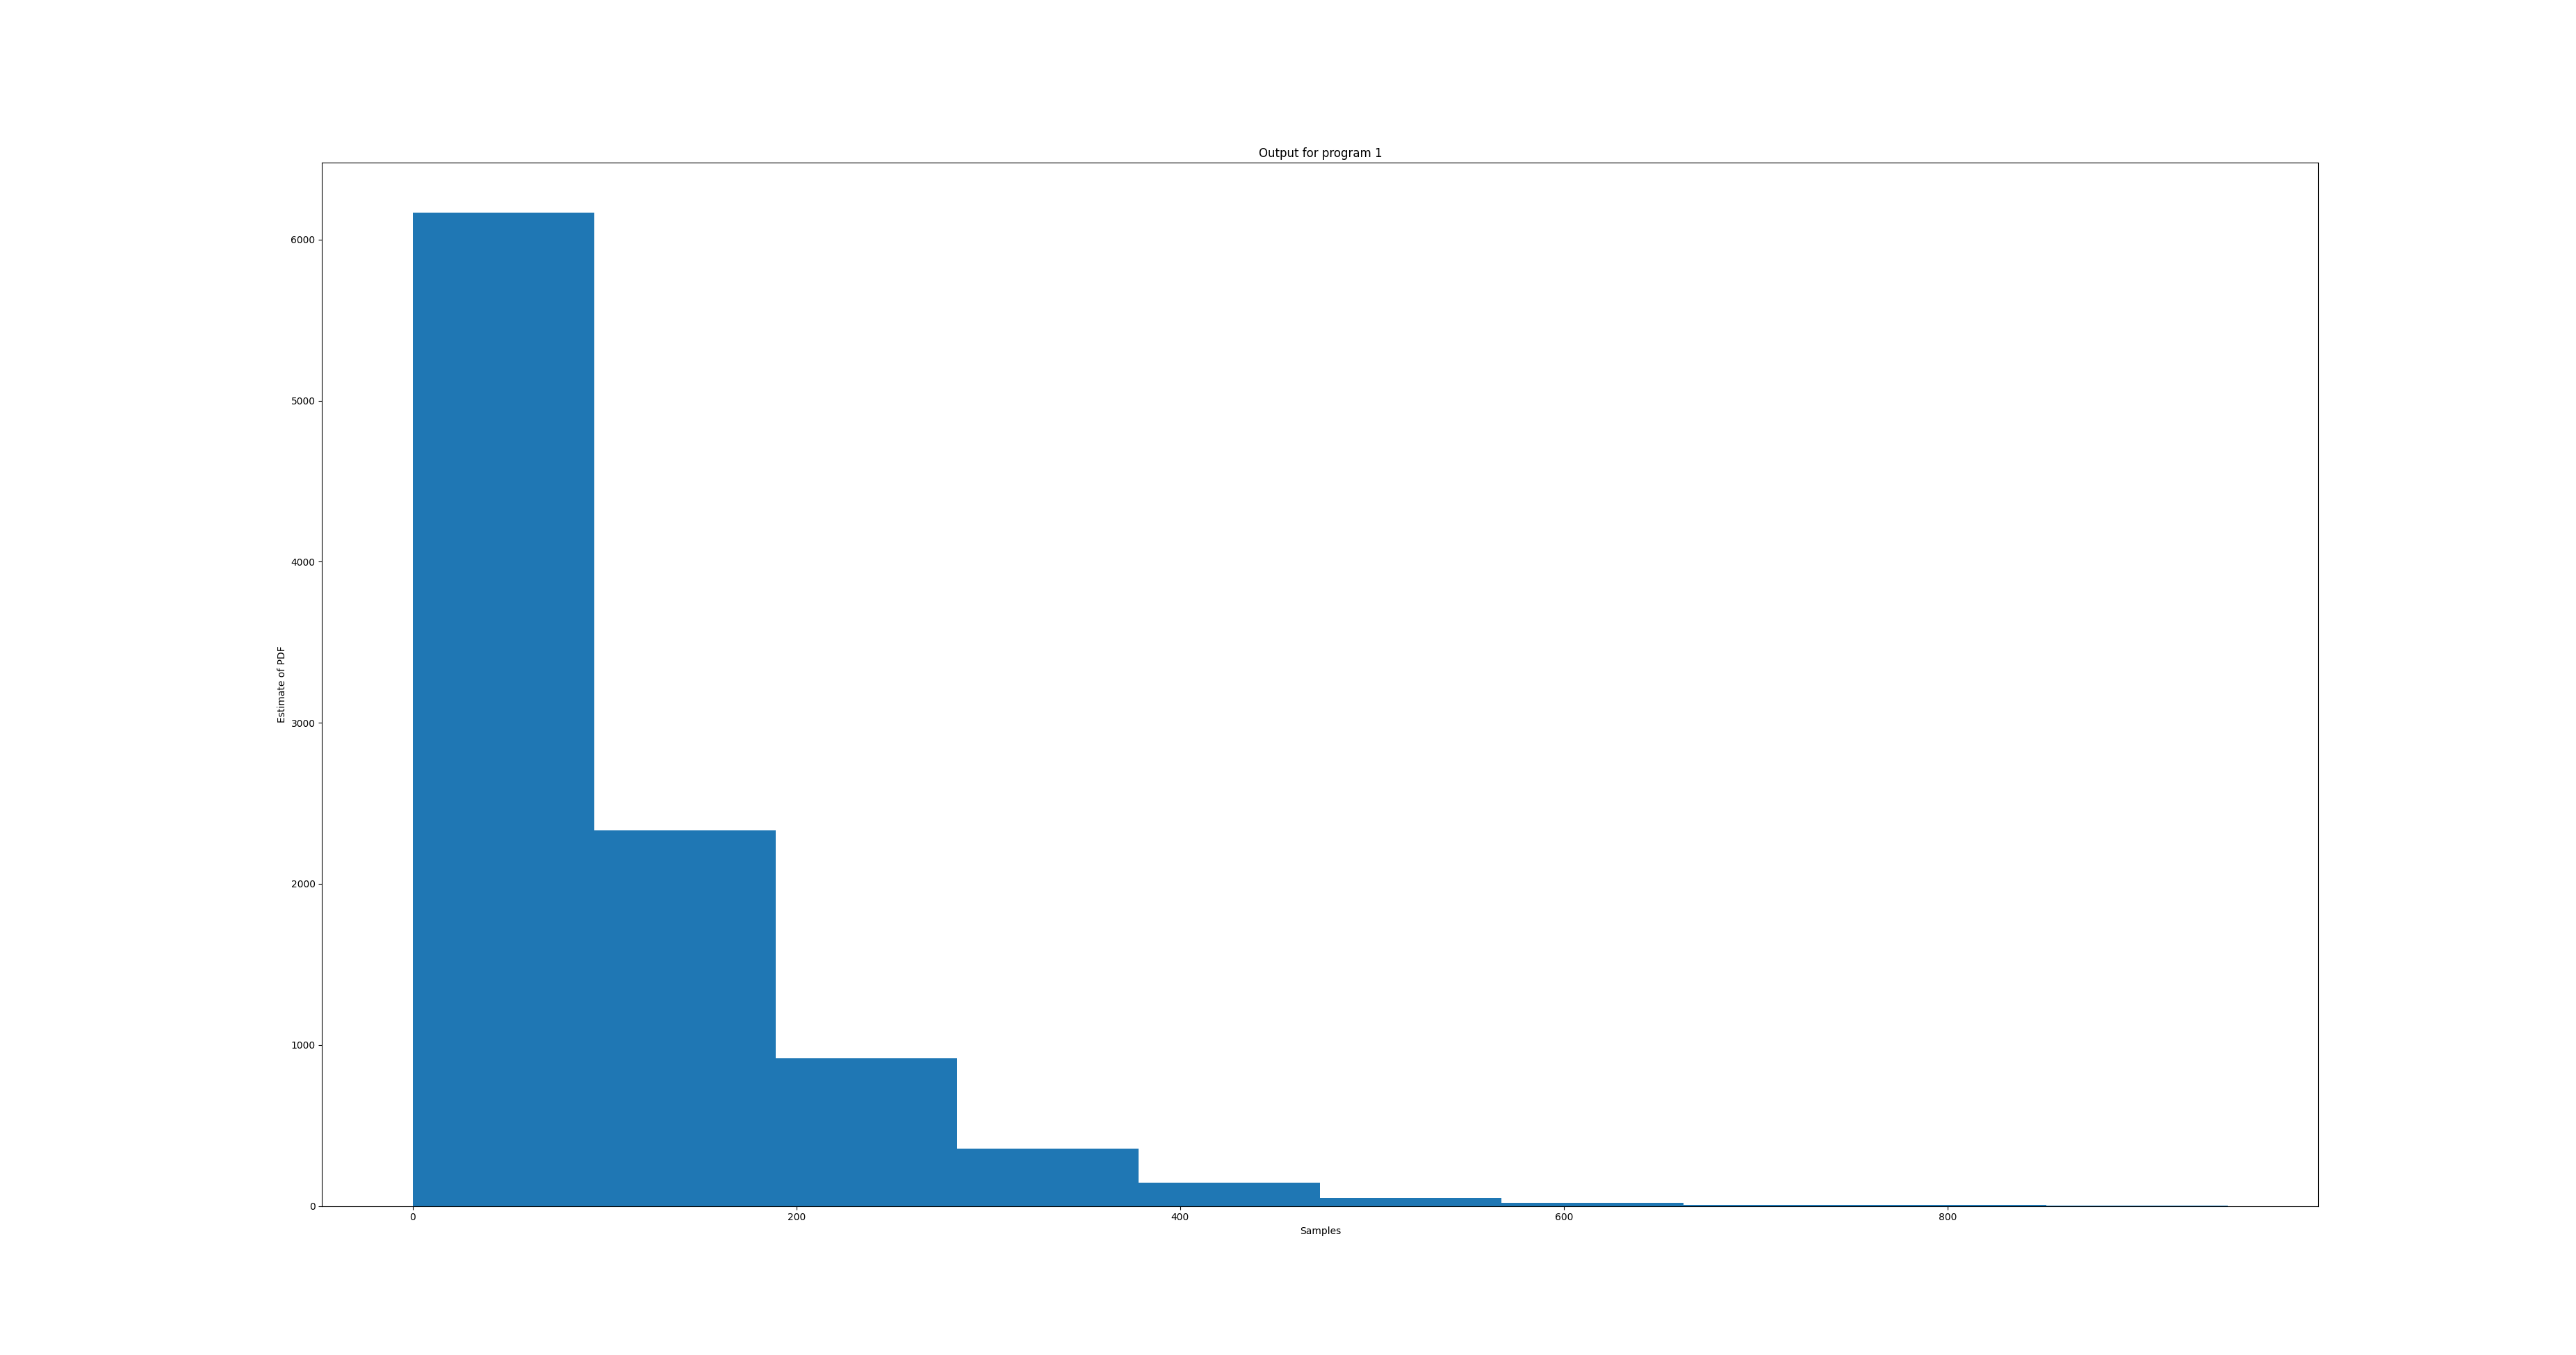
\includegraphics[width=\linewidth]{Figures/P1Hist.png}
	\captionof{figure}{Histogram for Program 1}
\end{center}

\subsection{Program 2}
Output from running program 2:
\begin{verbatim}
Sample of prior of program 2:
Elapsed time for program  2 .daphne is:  0:00:29.480438  seconds
Mean of samples:  tensor(0.9736)
Variance of samples:  tensor(5.0724)
\end{verbatim}
\begin{center}
	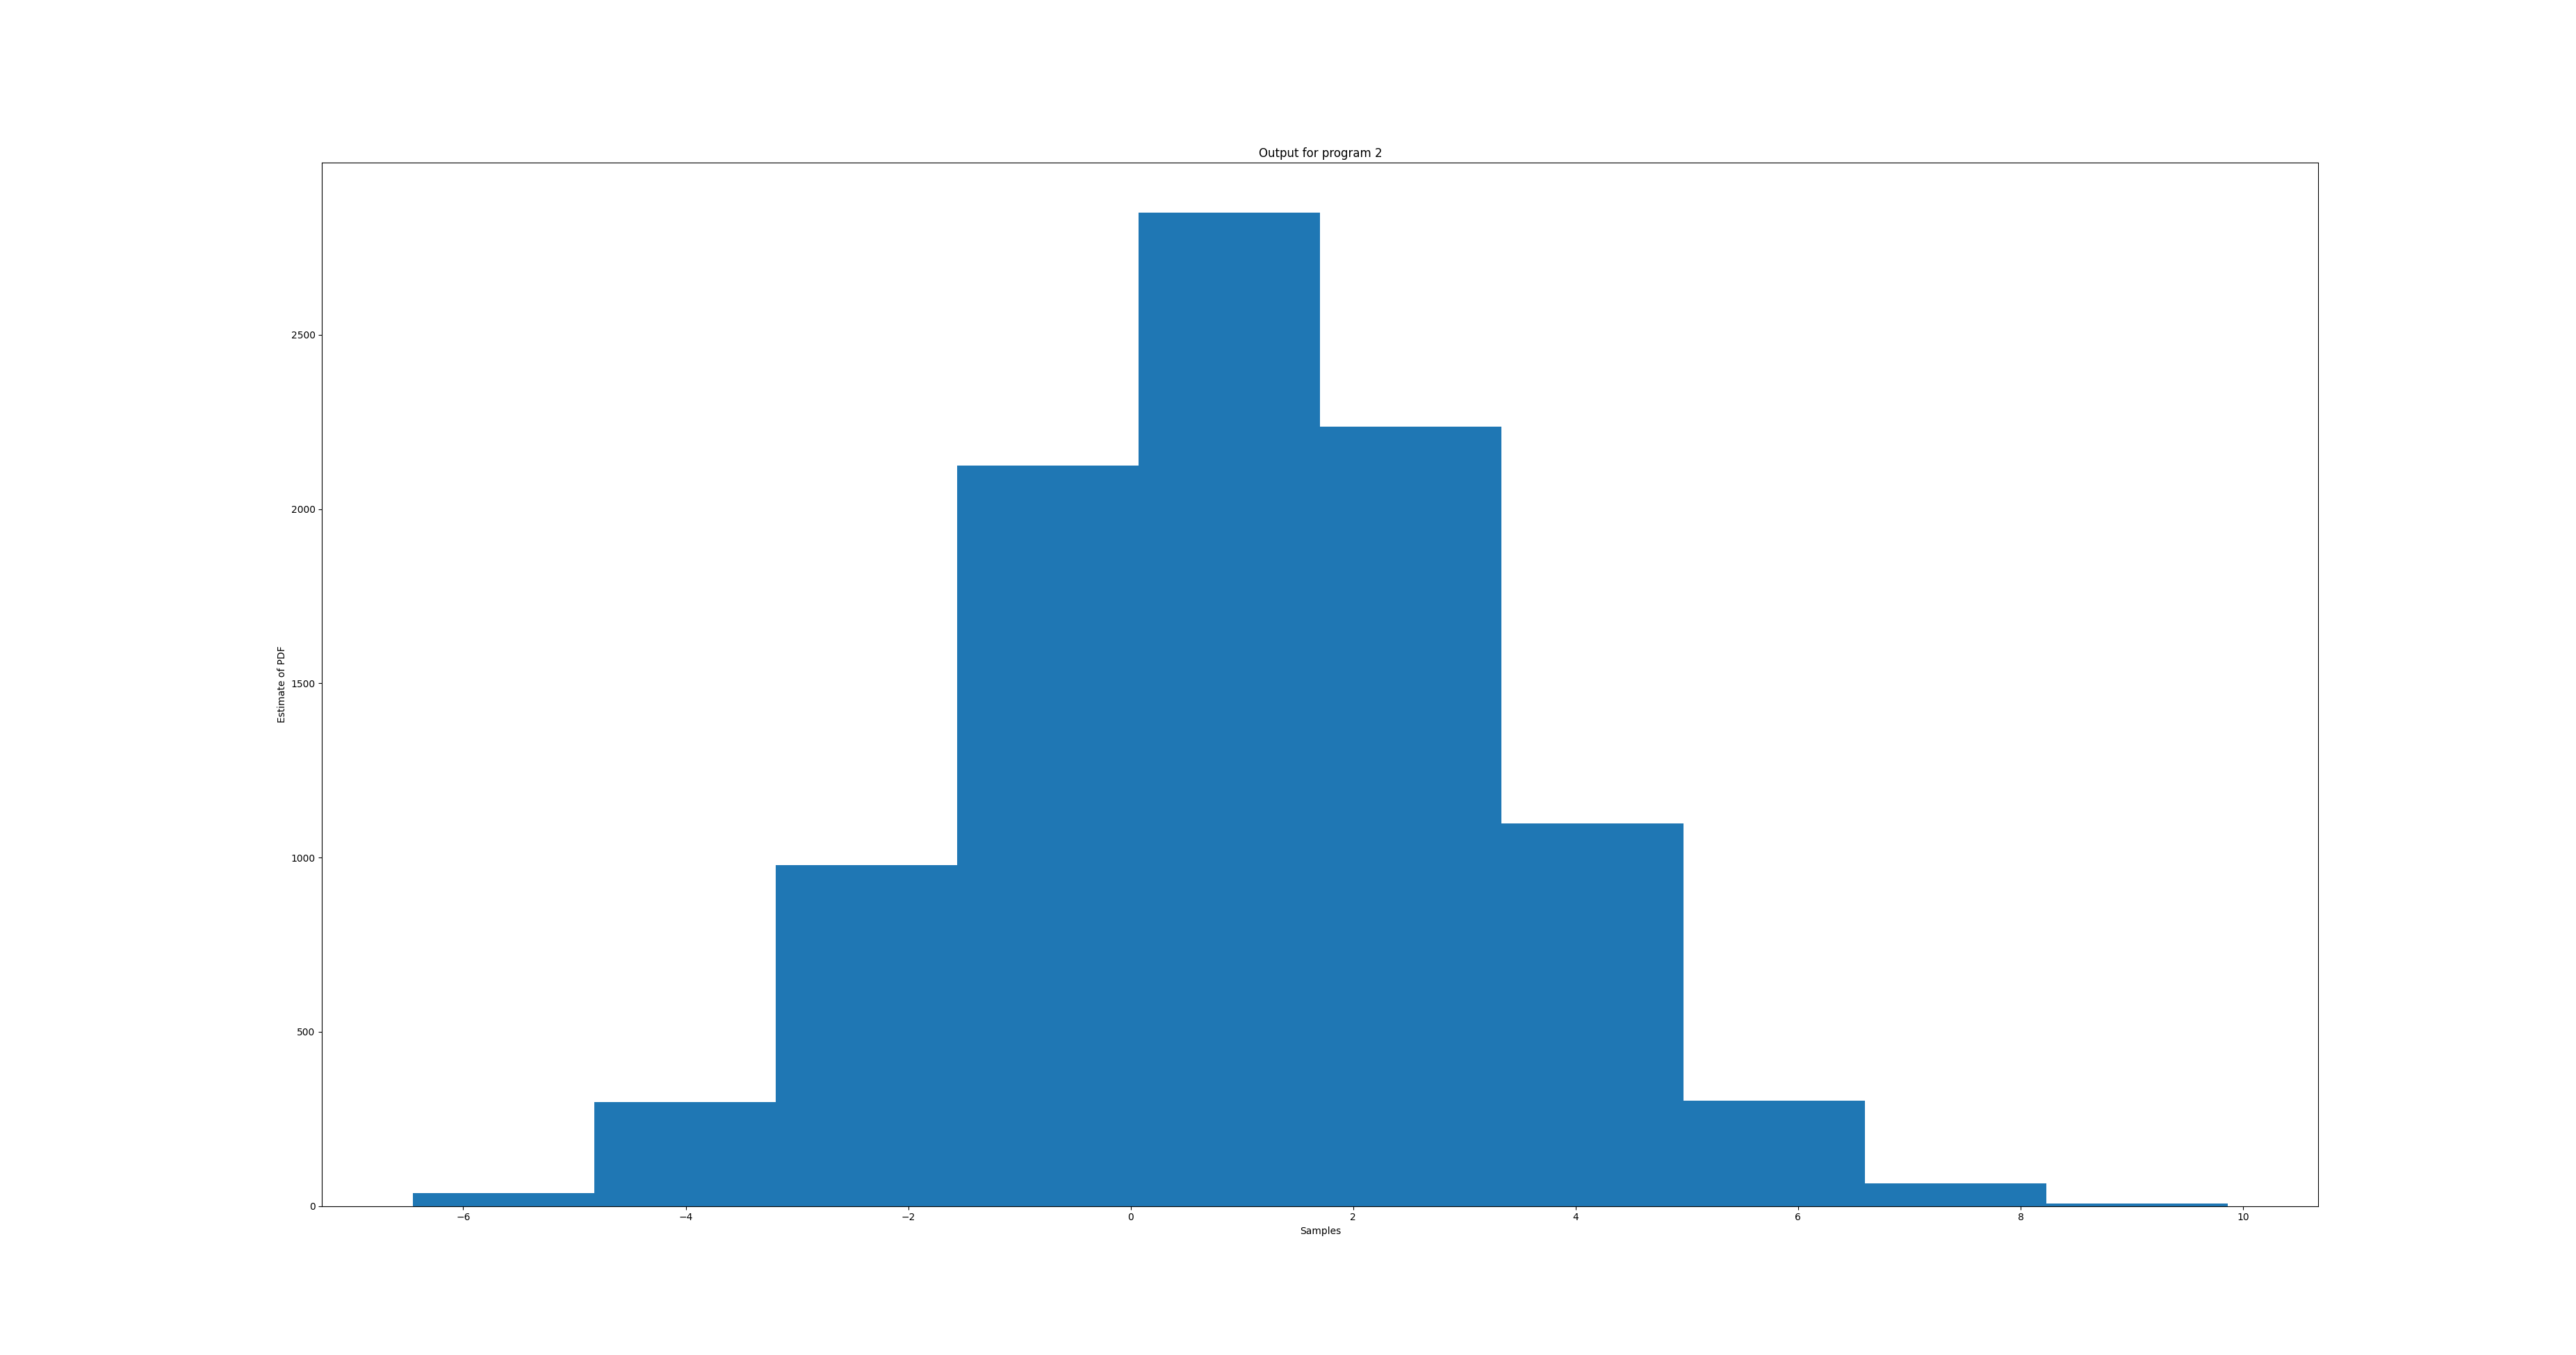
\includegraphics[width=\linewidth]{Figures/P2Hist.png}
	\captionof{figure}{Histogram for Program 2}
\end{center}

\subsection{Program 3}
Output from running program 3:
\begin{verbatim}
Sample of prior of program 3:
Elapsed time for program  3 .daphne is:  0:02:03.474374  seconds
\end{verbatim}
\begin{center}
	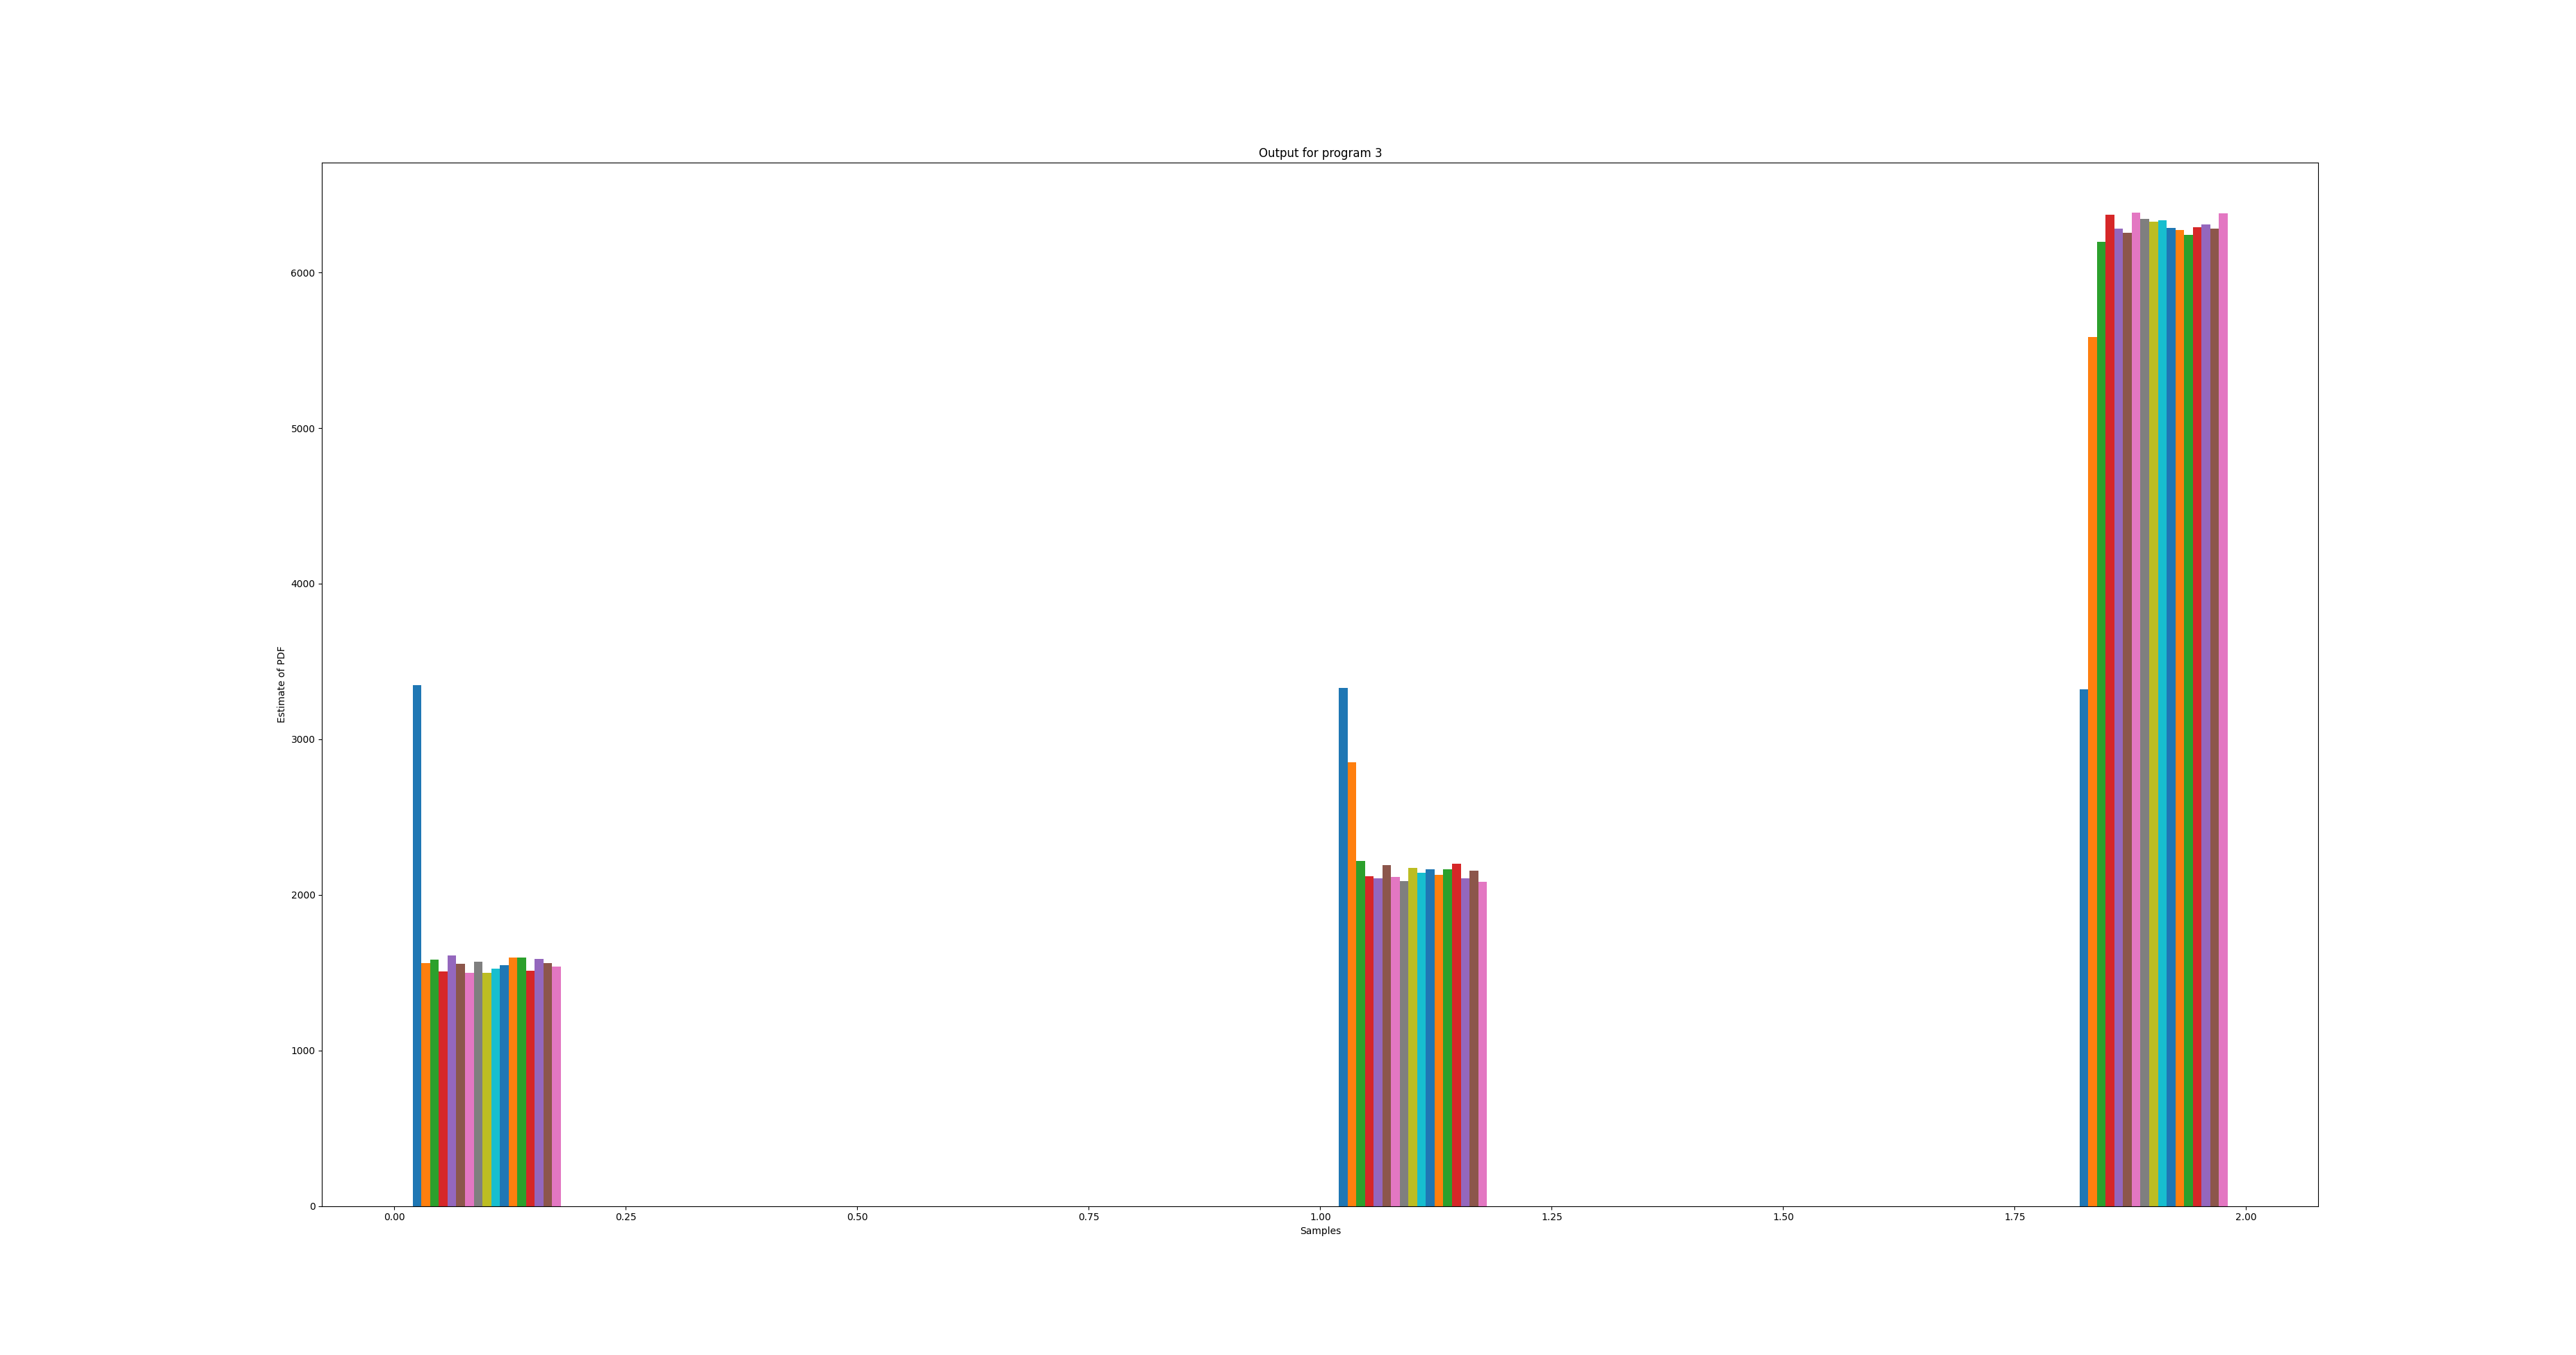
\includegraphics[width=\linewidth]{Figures/P3Hist.png}
	\captionof{figure}{Histogram for Program 3}
\end{center}
 
\end{document}
